
\section{Writing A Sample Barrelfish Application}

Here we show how to write a simple program on Barrelfish.  \textbf{XXX:} no
error handling yet.  Refer to \texttt{usr/tests/idctest} for code with proper
error handling.

\subsection{A Simple Hello World Program}

The source for user domains is stored under \begin{verbatim}/usr\end{verbatim}.

A simple hello world domain consists of a source file, and a Hakefile. e.g.,
\begin{verbatim}
usr/myapp
    myapp.c
    Hakefile
\end{verbatim}

For a simple hello world app, the source is trivial: a simple printf in main
will suffice (note that for output printf either uses a debug syscall to print
to the serial output, or a proper serial server if one is available).

\begin{verbatim}
#include <stdio.h>
int main(void) {
    printf("Hello World\n");
    return 0;
}
\end{verbatim}

To build the domain, call hake.sh in the build directory. This will create a
Config.hs, Makefile, and symbolic\_targets.mk. You can add myapp in the
symbolic\_tagets, then run make to build everything. You can also explicitly ask
make to build the domain. e.g.:
\begin{verbatim}
make x86_64/sbin/myapp
\end{verbatim}

After all is built, the menu.lst needs to be modified to add the domain and have
it started. Run everything in a simulator using:

\begin{verbatim}
make sim
\end{verbatim}

\section{A Simple Hello World Program Using IDC}

In this section, we talk how we can write an application that uses Barrelfish
IDC mechanism to communicate with other applications.  For purpose of this
section, we will develop simple \textbf{Hello World} client and server
application.  The client running on core-0 will send an IDC message to a
server running on core-1.  This message will contain a string with contents
\texttt{"Hello World"}.

Adding IDC (inter-dispatcher communication) is a bit more complicated. It
requires defining an interface in Flounder IDL, updating the interfaces
Hakefile, updating the domain's (myapp) Hakefile, and then adding initialization
code as well as appropriate callbacks to the source file.

\begin{figure}
  \begin{center}
    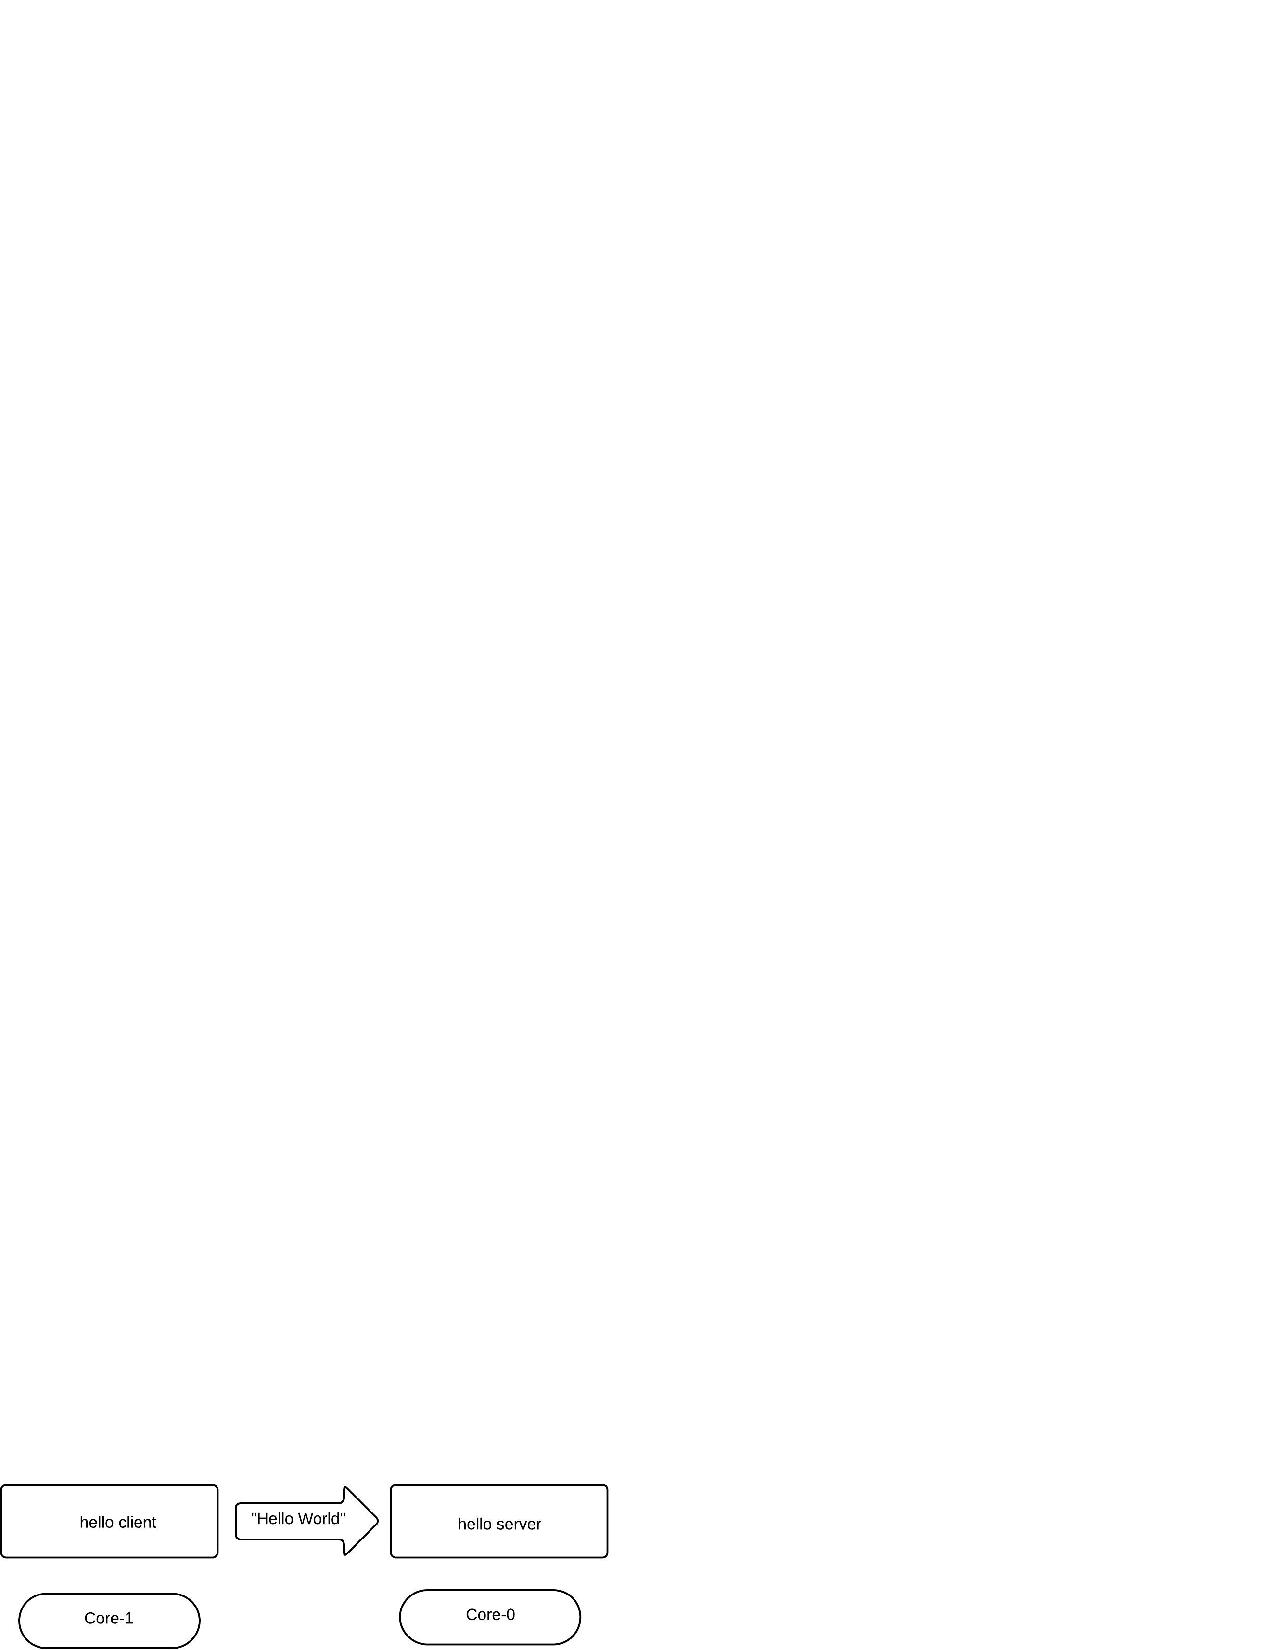
\includegraphics[width=0.8\columnwidth]{helloWorld2.pdf}
  \end{center}
  \caption{Hello world application overview}
  \label{fig:helloWorld}
\end{figure}

\subsection{Interface}

In this subsection, we will create a new interface
for our use.  We do this by creating a new interface file called
\texttt{hello.if} in the \texttt{if\\} directory. Following is simple interface
that will suffice for our requirements of sending single string as a message.


\verbatiminput{if/hello.if}
\begin{verbatim}
interface hello "Hello World interface" {
    message hello_msg(string s);
};
\end{verbatim}

You can find out more about how to write such interfaces by referring
\href{http://www.barrelfish.org/TN-011-IDC.pdf}{IDC-Technote}.

You also need to modify the \texttt{if/Hakefile} to add this newly created
interface into the compilation process.

\begin{verbatim}
[ flounderGenDefs (options arch) f
      | f <- [ "ahci_mgmt",
                ...
                ...
 	       "hello"],
             arch <- allArchitectures
] ++
\end{verbatim}

Adding the name of your interface here will make sure that the communication
stubs will be automatically generated for by the compilation process.  These
can be found in following location in your build directory:

\begin{verbatim}
BUILD/ARCH/include/if/hello_defs.h
BUILD/ARCH/include/if/hello_lmp_defs.h
BUILD/ARCH/include/if/hello_ump_defs.h
BUILD/ARCH/include/if/hello_multihop_defs.h
\end{verbatim}

There will be one for each type of communication mechanism supported by
the Barrelfish. You don't need to worry about these files as build mechanism
will take care of these files.  Only things developers need to do is
write the interface file and include appropriate headers in the application
code (discussed in following section)


\subsection{Application}

In this section, we discuss how would we write the application code,
and how to compile it.  For sake of simplicity, we will write both server and
client code in same application.  Following is the code for the \texttt{main}
function, which runs the client code or server code based on the
command line argument.


\begin{verbatim}
int main(int argc, char *argv[]) {
    errval_t err;
    if ((argc >= 2) && (strcmp(argv[1], "client") == 0)) {
        start_client();
    } else if ((argc >= 2) && (strcmp(argv[1], "server") == 0)) {
        start_server();
    } else {
        return EXIT_FAILURE;
    }
    /* The dispatch loop */
    struct waitset *ws = get_default_waitset();
    while (1) {
        err = event_dispatch(ws); /* get and handle next event */
        if (err_is_fail(err)) {
            DEBUG_ERR(err, "in event_dispatch");
            break;
        }
    }
    return EXIT_FAILURE;
}
\end{verbatim}

The important part of the above is in the dispatch loop where application
will wait for events on the default wait-set and handle those events
in infinite while loop.

\subsection{Server side}

In this section, we will develop the server code in steps of
"exporting service", "registering the service" and "handling actual requests".


\subsubsection{Exporting service}
As a first step, server needs to export the service it wants to provide
by calling export function on the service interface.  In this case, server
will call \texttt{hello\_export} as we are providing \textit{Hello World}
service.

\begin{verbatim}
static void start_server(void)
{
    errval_t err;
    err = hello_export(NULL /* state for callbacks */,
            export_cb, /* Callback for export */
            connect_cb,  /* Callback for client connects */
            get_default_waitset(), /* waitset where events will be sent */
            IDC_EXPORT_FLAGS_DEFAULT);
    if (err_is_fail(err)) {
        USER_PANIC_ERR(err, "export failed");
    }
}
\end{verbatim}

This call also registers two callback handles.  Once the service
is successfully exported, then the export callback provided.  When any client
connects with the service then the connect callback will be called.
We will see the use of these callbacks in next few steps.


\subsubsection{Registering service}
Server also need to register the service so that other applications can find
it.  Following code registers the \texttt{"hello\_service"} on the callback
from successful completion of export:


\begin{verbatim}
const static char *service_name = "hello_service";
static void export_cb(void *st, errval_t err, iref_t iref)
{
    if (err_is_fail(err)) {
        USER_PANIC_ERR(err, "export failed");
    }
    err = nameservice_register(service_name, iref);
    if (err_is_fail(err)) {
        USER_PANIC_ERR(err, "nameservice_register failed");
    }
}
\end{verbatim}

The \texttt{nameservice\_register} is a blocking call which will connect
to the global nameserver and publish the service name.

\subsubsection{Connect and handling messages}
This section describes how exactly the connection is established and
requests are handled.

\begin{verbatim}
static void rx_hello_msg(struct hello_binding *b, char *str)
{
    printf("server: received hello_msg:\n\t%s\n", str);
    free(str);
}

static struct hello_rx_vtbl rx_vtbl = {
    .hello_msg = rx_hello_msg,
};

static errval_t connect_cb(void *st, struct hello_binding *b)
{
    b->rx_vtbl = rx_vtbl;
    return SYS_ERR_OK;
}
\end{verbatim}

The above code defines a function \texttt{rx\_hello\_msg} which will be
responsible to actually handle the requests.  In our case, we are just
printing out the string we received as part of the message.

We need to create a list of function pointers where one function pointer
is assigned for every possible incoming message. So we are creating
an instance \texttt{rx\_vtbl} of type \texttt{hello\_rx\_vtbl}.

On arrival of new connection, we provide this list of function pointers
to register which functions to call for handling particular type of message.


\subsection{Client side}
Client needs to find the service and connect to it.  Once the connection
is successfully established then it can send the actual requests. In this
section, we show how it can be done.


\subsubsection{Find and Bind}
Following code finds the desired service with given name and binds with
the service.

\begin{verbatim}
static void start_client(void)
{
    errval_t err;
    iref_t iref;
    err = nameservice_blocking_lookup(service_name,
            &iref);
    if (err_is_fail(err)) {
        USER_PANIC_ERR(err,
                "nameservice_blocking_lookup failed");
    }
    err = hello_bind(iref, bind_cb, /* Callback function */
            NULL /* State for the callback */,
            get_default_waitset(),
            IDC_BIND_FLAGS_DEFAULT);
    if (err_is_fail(err)) {
        USER_PANIC_ERR(err, "bind failed");
    }
}
\end{verbatim}

As the name suggests  \texttt{nameservice\_blocking\_lookup} is a blocking
call which will connect with the nameserver and query for the given
service name.  The \texttt{iref} handle returned by this call can be used
for binding with the service.

The \texttt{hello\_bind} is part of the code generated from the interface
file and will try and connect with the server on appropriate channel.

Following code is callback function which will be called when client
successfully connects with the server.  This code also creates a client
state which stores pointer to the communication channel binding.  This code
then calls a function \texttt{run\_client} with the client state.


\begin{verbatim}
struct client_state {
    struct hello_binding *binding;
    int count;
};

static void bind_cb(void *st, errval_t err, struct hello_binding *b)
{
    struct client_state *myst = malloc(sizeof(struct client_state));
    assert(myst != NULL);
    myst->binding = b;
    myst->count = 0;
    run_client(myst);   /* calling run_client for first time */
}
\end{verbatim}


\subsubsection{Sending messages}

Most of the actual work of sending message is done from the \texttt{run\_client}
function which is described bellow:

\begin{verbatim}
static void run_client(void *arg)
{
    errval_t err;
    struct client_state *myst = arg;
    struct hello_binding *b = myst->binding;

    /* Creating a continuation which will call run_client */
    struct event_closure txcont = MKCONT(run_client, myst);

    err = b->tx_vtbl.hello_msg(b, txcont, "Hello World");
    if (err_is_fail(err)) {
        DEBUG_ERR(err, "error sending message %d\n", myst->count);
    }
}
\end{verbatim}

This function first creates a continuation which calls itself
and will be used as a callback function. The next step is to actually
send the message by calling an appropriate function on the send side of
interface binding (\texttt{tx\_vtbl.hello\_msg}) with actual message
and above created continuation.  This call will register a message to be sent
and a callback that will be triggered when message is successfully.

As you can notice, callback function is calling \texttt{run\_client} again,
leading an infinite loop of sending messages.

\subsubsection{Include files}

Following is a typical set of include files that you will need to add
in your code.

\begin{verbatim}
#include <stdio.h>
#include <barrelfish/barrelfish.h>
#include <barrelfish/nameservice_client.h>
#include <if/hello_defs.h>
\end{verbatim}

The \texttt{barrelfish.h} file contains declaration of
functionalities related to Barrelfish OS (eg: system calls, capability
system related functionalities, etc.)
\texttt{nameservice\_client.h} file provides declarations for functions related
to registering and looking up services.  The \texttt{hello\_defs.h} file
includes the declarations for automatically generated code to support
\texttt{if/hello.if} interface.


\subsection{Building and running the application}

In this section, we talk about how build your application.  For this, you
will need to create a \texttt{Hakefile} in the code directory which should
look something like bellow:

\begin{verbatim}
    [ build application { target = "hello-cs",
                          cFiles = [ "hello.c" ],
                          flounderBindings = [ "hello" ]
                        }
    ]
\end{verbatim}

This \texttt{Hakefile} specifies that you want to build an application
with name \texttt{hello\-cs} from the \texttt{hello.c} file, and also
it marks the dependency on the communication interface \texttt{hello}.

The next step is to modify the \texttt{barrelfish/hake/symbolic\_targets.mk}
file to include your newly created application into the build process.
Here you can choose an architecture for which your application should be
compiled, or you can also add your application in \texttt{MODULES\_COMMON}
list so that your application will be compiled for all architectures.

\begin{verbatim}
MODULES_COMMON= \
	sbin/init_null \
        ...
        ...
	sbin/xcorecapbench \
	sbin/hello-cs \

\end{verbatim}

After this, rebuild the Barrelfish to include newly added application.  On
successful compilation the binary will be created in sbin directory of
desired architecture.


% ########### Editing menu.lst
Next step is to edit one of the \texttt{barrelfish/hake/menu.lst.*} file based
on which architecture you are targeting.  Bellow is the minimal
\texttt{menu.lst.x86\_64} file to be able to run this newly created application.

\begin{verbatim}
title	Barrelfish
root	(nd)
kernel	/x86_64/sbin/elver loglevel=4
module	/x86_64/sbin/cpu loglevel=4
module	/x86_64/sbin/init

# Domains spawned by init
module	/x86_64/sbin/mem_serv
module	/x86_64/sbin/monitor

# Special boot time domains spawned by monitor
module  /x86_64/sbin/ramfsd boot
module  /x86_64/sbin/skb boot
modulenounzip /skb_ramfs.cpio.gz nospawn
module  /x86_64/sbin/kaluga boot
module  /x86_64/sbin/acpi boot
module  /x86_64/sbin/spawnd boot
#bootapic-x86_64=1-15
module  /x86_64/sbin/startd boot
module /x86_64/sbin/routing_setup boot

# Drivers
module /x86_64/sbin/pci auto
module /x86_64/sbin/ahcid auto

# General user domains
module	/x86_64/sbin/serial

# Your hello world application (both server and client)
module /x86_64/sbin/hello-cs core=0 server
module /x86_64/sbin/hello-cs core=1 client
\end{verbatim}

Now, you can build your application and verify that binary is created as
follows:

\begin{verbatim}
$ make
$ ls x86_64/sbin/hello-cs
\end{verbatim}

If everything goes fine, you can run the application in \texttt{qemu} simulator
with following command:
\begin{verbatim}
$ make sim
\end{verbatim}

At this moment, you should be able see Barrelfish booting and starting your
applications which are then able to communicate by sending "Hello World"
message in infinite loop.  Following is a sample output that you may expect
while running this setup.

\begin{verbatim}
...
...
...
startd.0: starting app /x86_64/sbin/hello-cs on core 0
spawnd.0: spawning /x86_64/sbin/hello-cs on core 0
startd.0: starting app /x86_64/sbin/hello-cs on core 1
skb.0: waiting for: spawn.1
skb.0: waiting for: pci
spawnd.0: spawning /x86_64/sbin/ahcid on core 0
kernel: 0: installing handler for IRQ 1
kernel: 0: installing handler for IRQ 2
pci_client.c: got vector 2
ahcid: registered device 8086:2922
spawnd.1: spawning /x86_64/sbin/hello-cs on core 1
No bootscript
server: received hello_msg:
        Hello World
server: received hello_msg:
        Hello World
server: received hello_msg:
        Hello World
server: received hello_msg:
        Hello World
server: received hello_msg:
        Hello World
server: received hello_msg:
        Hello World
...
...
...
\end{verbatim}


